\documentclass[
  bibliography=totoc,     % Literatur im Inhaltsverzeichnis
  captions=tableheading,  % Tabellenüberschriften
  titlepage=firstiscover, % Titelseite ist Deckblatt
]{scrartcl}

% Paket float verbessern
\usepackage{scrhack}

% Warnung, falls nochmal kompiliert werden muss
\usepackage[aux]{rerunfilecheck}

% unverzichtbare Mathe-Befehle
\usepackage{amsmath}
% viele Mathe-Symbole
\usepackage{amssymb}
% Erweiterungen für amsmath
\usepackage{mathtools}

% Fonteinstellungen
\usepackage{fontspec}
% Latin Modern Fonts werden automatisch geladen
% Alternativ zum Beispiel:
%\setromanfont{Libertinus Serif}
%\setsansfont{Libertinus Sans}
%\setmonofont{Libertinus Mono}

% Wenn man andere Schriftarten gesetzt hat,
% sollte man das Seiten-Layout neu berechnen lassen
\recalctypearea{}

% deutsche Spracheinstellungen
\usepackage{polyglossia}
\setmainlanguage{german}


\usepackage[
  math-style=ISO,    % ┐
  bold-style=ISO,    % │
  sans-style=italic, % │ ISO-Standard folgen
  nabla=upright,     % │
  partial=upright,   % ┘
  warnings-off={           % ┐
    mathtools-colon,       % │ unnötige Warnungen ausschalten
    mathtools-overbracket, % │
  },                       % ┘
]{unicode-math}

% traditionelle Fonts für Mathematik
\setmathfont{Latin Modern Math}
% Alternativ zum Beispiel:
%\setmathfont{Libertinus Math}

\setmathfont{XITS Math}[range={scr, bfscr}]
\setmathfont{XITS Math}[range={cal, bfcal}, StylisticSet=1]

% Zahlen und Einheiten
\usepackage[
  locale=DE,                   % deutsche Einstellungen
  separate-uncertainty=true,   % immer Fehler mit \pm
  per-mode=symbol-or-fraction, % / in inline math, fraction in display math
]{siunitx}

% chemische Formeln
\usepackage[
  version=4,
  math-greek=default, % ┐ mit unicode-math zusammenarbeiten
  text-greek=default, % ┘
]{mhchem}

% richtige Anführungszeichen
\usepackage[autostyle]{csquotes}

% schöne Brüche im Text
\usepackage{xfrac}

% Standardplatzierung für Floats einstellen
\usepackage{float}
\floatplacement{figure}{htbp}
\floatplacement{table}{htbp}

% Floats innerhalb einer Section halten
\usepackage[
  section, % Floats innerhalb der Section halten
  below,   % unterhalb der Section aber auf der selben Seite ist ok
]{placeins}

% Seite drehen für breite Tabellen: landscape Umgebung
\usepackage{pdflscape}

% Captions schöner machen.
\usepackage[
  labelfont=bf,        % Tabelle x: Abbildung y: ist jetzt fett
  font=small,          % Schrift etwas kleiner als Dokument
  width=0.9\textwidth, % maximale Breite einer Caption schmaler
]{caption}
% subfigure, subtable, subref
\usepackage{subcaption}

% Grafiken können eingebunden werden
\usepackage{graphicx}
% größere Variation von Dateinamen möglich
\usepackage{grffile}

% schöne Tabellen
\usepackage{booktabs}

% Verbesserungen am Schriftbild
\usepackage{microtype}

% Literaturverzeichnis
\usepackage[
  backend=biber,
]{biblatex}
% Quellendatenbank
\addbibresource{lit.bib}
\addbibresource{programme.bib}

% Hyperlinks im Dokument
\usepackage[
  unicode,        % Unicode in PDF-Attributen erlauben
  pdfusetitle,    % Titel, Autoren und Datum als PDF-Attribute
  pdfcreator={},  % ┐ PDF-Attribute säubern
  pdfproducer={}, % ┘
]{hyperref}
% erweiterte Bookmarks im PDF
\usepackage{bookmark}

% Trennung von Wörtern mit Strichen
\usepackage[shortcuts]{extdash}

\author{%
  Jan Philipp Jäkel\\%
  \href{mailto:jan.jaekel@tu-dortmund.de}{jan.jaekel@tu-dortmund.de}%
  \texorpdfstring{\and}{,}%
  Piet Hoffmann\\%
  \href{mailto:piet.hoffmann@tu-dortmund.de}{piet.hoffmann@tu-dortmund.de}%
}
\publishers{TU Dortmund – Fakultät Physik}


\subject{V353}
\title{Relaxationsverhalten eines RC-Kreises}

\date{
  \begin{align}
    \text{Durchführung: } & \text{19.12.2017} & \hspace{3em} & \text{Abgabe: 9.1.2018} \notag
%\\  \text{Korrektur: } & \text{22.11.2017} & \hspace {3em} & \notag 
  \end{align}
}

%\date{%
%  Durchführung: DATUM
%  \hspace{3em}
%  Abgabe: DATUM
%}

\begin{document}

\maketitle
\thispagestyle{empty}
\tableofcontents
\newpage

\section{Zielsetzung}
Im allgeminen soll das Relaxationsverhalten eines RC-Schwingkreises untersucht werden.
Dabei wird die Phasenabhängigkeit des Schwingkreises beobachtet und überprüft ob der RC-Schwingkreis als Integrator fungieren kann.

\section{Theorie}
\label{sec:Theorie}
\subsection{Die allgemine Relaxationsgleichung}
Wenn ein System ausgelenkt wird und nicht oszillatorisch in seinen Anfangszustand zurückkehrt, treten Relaxationserscheinungen auf.
Die Geschwindigkeit der Rückkehr ist dabei proportional zu der Auslenkung:
\begin{equation}
  \frac{dA}{dt}=c[A(t)-A(\infty)]
\end{equation}
Durch Integration von $0$ bis $t$ ergibt sich:
\begin{equation}
  \ln{\frac{A(t)-A(\infty)}{A(0)-A(\infty)}}=ct
\end{equation}
Wird die e-Funktion auf die Gleichung anngewendet ergibt sich:
\begin{equation}
  \label{eq:gl2}
  A(t)=A(\infty)+[A(0)-A(\infty)]\exp(ct)
\end{equation}
Wobei $c<0$ sein muss, damit $A$ beschränkt ist.
\subsection{Anwendung auf den Auf- und Entladevorgag des RC-Schwingkreises}
Der in Abbildung befindliche Kondensator soll aufgeladen sein, dann liegt zwischen den Platten eine Spanung
\begin{equation}
  U_C=\frac{Q}{C}
\end{equation}
an.
Nach dem ohmschen Gesetz lässt sich der Strom durch
\begin{equation}
  I = \frac{U_C}{R}
\end{equation}
ausdrücken.
Damit findet sich für den zeitlichen Verlauf der Ladung folgende Dgl.:
\begin{equation}
  \frac{dQ}{dt}=\frac{1}{RC}Q(t)
\end{equation}
Mit $Q(\infty)=0$ ergibt sich analog zu der Gleichung\eqref{eq:gl2}:
\begin{equation}
  Q(t)=Q(0)\exp(\frac{-t}{RC})
\end{equation}
Für den Aufladevorgang gelten die Randbedingungen
\begin{equation}
  Q(0)=0
\end{equation}
und
\begin{equation}
  Q(\infty)=CU_0 .
\end{equation}
Damit folgt für den Zeitlichhen Verlauf der Ladung:
\begin{equation}
  Q(t) = CU_0 \exp(\frac{-t}{RC})
\end{equation}
Die Zeitkonstante ist ein Maß für die Geschwindigkeit der Relaxation des Systems. Hier ist diese $\frac{1}{RC}$.

\subsection{Auf- und Entladevorgag mit periodischer Anregung}
Liegt eine Wechselspannung
\begin{equation}
  U(t)=U_0 cos(\omega t)
\end{equation}
an, so lässt sich mit folgendem Ansatz eine Lösung für das Problem finden:
\begin{equation}
  U_c(t)= A(\omega) \cos{(\omega t + \phi(\omega))}
\end{equation}
Damit gilt für den Stromkreis, unter einbezug des zweiten Kirchhoffschen Gesetzes:
\begin{equation}
  \label{eq:gl3}
  U_0 \cos{(\omega t)} = A \omega R C \sin{(\omega t + \phi)} + A(\omega)\cos{(\omega t + \phi)}
\end{equation}
Gleichung \eqref{eq:gl3} muss für alle $t$ gelten. Mit $\omega t= \frac{\pi}{2}$ ergibt sich dann:
\begin{equation}
  0 = - \omega R C \sin{(\frac{\pi}{2}+\phi)} + \cos{(\frac{\pi}{2}+\phi)}
\end{equation}
Durch umformung ergibt sich dann folgende Beziehung für die Phasenverschiebung:
\begin{equation}
  \phi(\omega)=\arctan{(- \omega R C)}
\end{equation}
Mit $\omega +\phi =\frac{\pi}{2}$ ergibt sich für die Generatorspannung:
\begin{equation}
  \label{eq:gl4}
  A(\omega)= \frac{U_0}{\sqrt{1+\omega^2 R^2 C^2}}
\end{equation}
Es ist durch Gleichung\eqref{eq:gl4} erkennbar, dass das RC-Glied ein Tiefpass ist.

\subsection{Der RC-Kreis als Integrator}
Es gilt:
\begin{equation}
  U(t)= RC \frac{dU_c}{dt} + U_c(t)
\end{equation}
Unter der Voraussetzung $\omega \gg\frac{1}{RC}$ ist $|U_C| \ll|U|$.
Somit lässt sich näherungsweise
\begin{equation}
  U(t)=RC \frac{dU_C}{dt}
\end{equation}
schreiben.
Anders lässt sich dies als
\begin{equation}
  U_C(t)=\int_0^t U(t') dt
\end{equation}
schreiben.
Die am Kondensator anliegende Spannung ist also proportional zu dem Integral der Generatorspannung.

\section{Durchführung}
\label{sec:Durchführung}
\subsection{Auf- und Entladevorgang}
Um den Auf- und Entladevorgang zu untersuchen wird folgendes Schaltbild aufgebaut.
\begin{figure}[H]
    \centering
    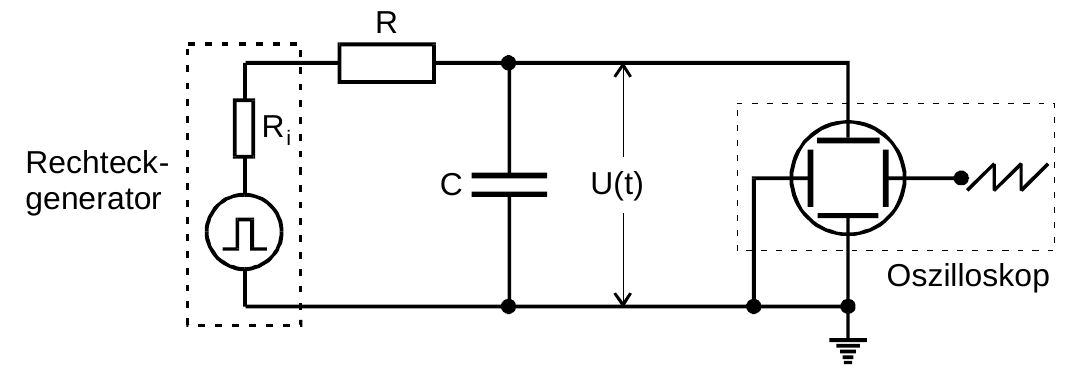
\includegraphics[width=\textwidth]{content/aufbau1.png}
    \caption{Aufbau der ersten Messung.\cite{v353}}
    \label{fig:mess1}
\end{figure}
\noindent
Dabei wird das RC-Glied an einen Rechteckgenerator angeschlossen und die resultierende Kondensatorspannung $U_C$ mit einem Oszilloskop beobachtet, sodass sich ein stationäres Bild einstellt. Die Spannung wird zu mehreren Zeitpunkten innerhalb der Periode bei einer geeineten Frequenz abgelesen.
Im Allgemeinen ist der Innenwiderstand des Generators zu beachten, welcher mit \mbox{$R_i=\SI{600}{\ohm}$\cite{v353}} angegeben ist. Wenn jedoch der Widerstand des RC-Glieds ausreichend hoch ist, kann ersterer vernachlässigt werden. Daher muss $R$ ausgemessen werden, um die Ergebnisse des Versuchs beurteilen zu können.
%
\subsection{Frequenzabhängigkeit der Amplitude}
Es wird die Frequenzabhängigkeit der Amplitude der Kondensatorspannung bei Sinusförmiger Anregung des RC-Glieds untersucht.
Dafür wird die Schaltung wie in Abbildung \ref{fig:mess2} gezeigt aufgebaut.
\begin{figure}[H]
    \centering
    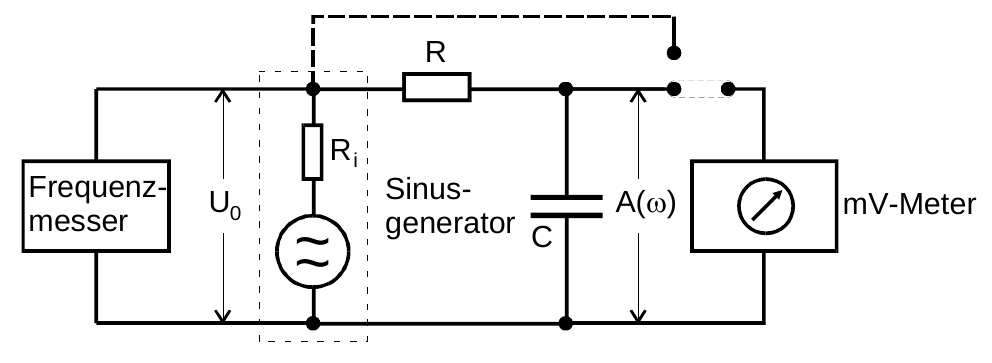
\includegraphics[width=\textwidth]{content/aufbau2.png}
    \caption{Aufbau der zweiten Messung.\cite{v353}}
    \label{fig:mess2}
\end{figure}
\noindent
Anstatt des Rechteckgenerators wird nun ein Sinusgenerator verwendet. Dieser wird im Verlauf der Messung auf verschiedene Frequenzen über mehrere Zehnerpotenzen hinweg eingestellt und die resultierende Amplitude des Kondensatorspannung gemessen.
Auch hier ist der Innenwiderstand des Generators zu beachten.
%
\subsection{Frequenzabhängigkeit der Phasenverschiebung}
Im Gegensatz zur vorausgegangenen Messung wird nun auch die Generatorspannung gleichzeitig mit dem Oszilloskop beobachtet, sodass sich die Phasenverschiebung zwischen beiden messen lässt.
\begin{figure}[H]
    \centering
    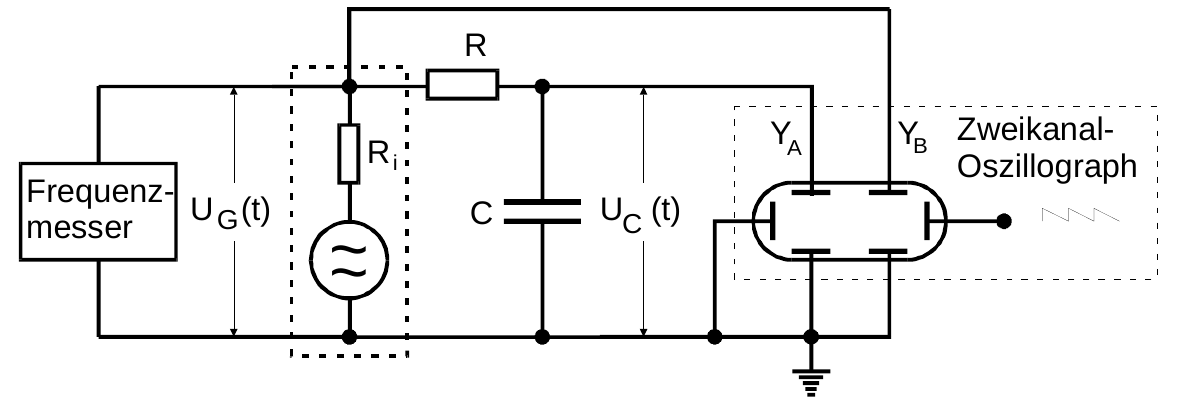
\includegraphics[width=\textwidth]{content/aufbau3.png}
    \caption{Aufbau der zweiten Messung.\cite{v353}}
    \label{fig:mess3}
\end{figure}
\noindent
Da sich der Phasenwinkel nicht direkt ablesen lässt wird einerseits der zeitliche Abstand zwischen zwei entsprechenden Nulldurchgängen beider Spannungssignale, hier $a$, und zusätzlich die gesamte Periode, hier $b$, gemessen, woraus sich der Phasenwinkel nach
\begin{equation}
    \phi = 2\pi \, \frac{a}{b} 
    \label{eqn:abphase}
\end{equation}
ergibt.
Auch hier wird Frequenz des Generators im Verlauf der Messreihe über mehrere Zehnerpotenzen variiert.

\section{Auswertung}
\label{sec:Auswertung}
\subsection{Bestimmung des RC-Glieds}
Die Messung wird wie in der Duchtführung beschrieben durchgeführt.
Die so erhaltenen Messwerte befinden sich in Tabelle\ref{tab:Messwerte1} :
\begin{table}[H]
    \centering
    \caption{Kondensatorspannung bei fester Frequenz.}
    \label{tab:Messwerte1}
    \begin{tabular}{S[table-format=1.1] S[table-format=2.2] }
        \toprule
        {$t/\si{\milli\second}$} & {$U_C/\si{\volt}$} \\
        \midrule
        0.2 & 14.00 \\
        0.4 & 11.10 \\
        0.6 & 8.64  \\
        0.8 & 6.72  \\
        1.0 & 5.36  \\
        1.2 & 4.08  \\
        1.4 & 3.20  \\
        1.6 & 2.48  \\
        1.8 & 1.92  \\
        2.0 & 1.60  \\
        2.2 & 1.28  \\
        2.4 & 0.96  \\

        \bottomrule
    \end{tabular}
\end{table}

\noindent Die Messwerte werden in der halblogarithmischen Abbildung aufgetragen.
Es wird eine lineare Ausgleichsrechnung, mit Python, durchgeführt und aufgetragen.
Diese hat eine Steigung von $m=\SI{-1.03\pm0.14}{\per\milli\second}$
und einen $y$-Achsenabschnitt von $b=(2.75\pm0.19)$.

\begin{figure}
    \centering
    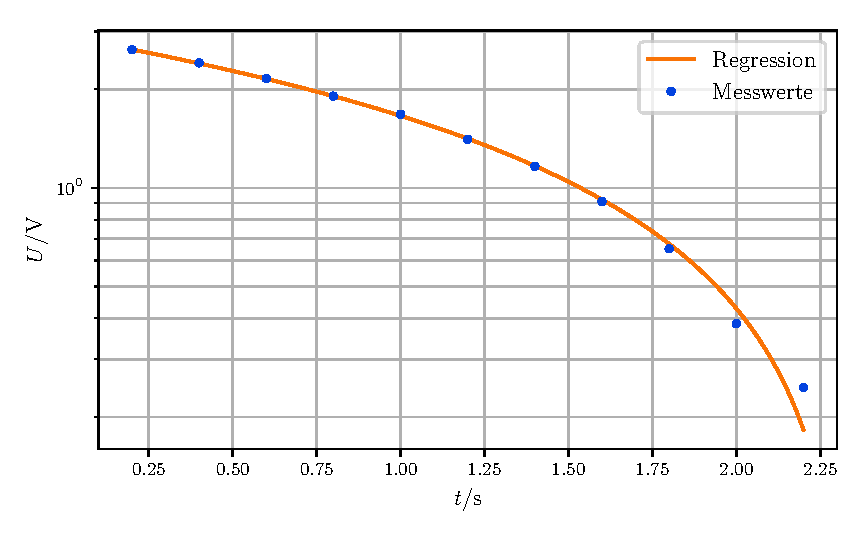
\includegraphics[width=\textwidth]{build/messung1.pdf}
    \caption{Messwerte und Ausgleichsgerade.}
    \label{fig:plot1}
\end{figure}

Die Steigung ist hier $\frac{1}{RC}$ .
Damit ist $RC$ der Kehrwert der Steigung.
\begin{equation*}
  RC=\SI{0.97\pm0.14}{\milli\second}
\end{equation*}
\subsection{Frequenzabhängigkeit der Kondensatorspannung}
Die Messung wird wie in der Durchführung beschrieben ausgeführt.
Die so erhaltenen Messwerte befinden sich in Tabelle\ref{tab:Messwerte2}:
\begin{table}[H]
    \centering
    \caption{Kondensatorspannung bei variabler Frequenz.}
    \label{tab:Messwerte2}
    \begin{tabular}{S[table-format=6.2] S[table-format=2.3] }
        \toprule
        {$f/\si{\hertz}$} & {$U_C/\si{\volt}$} \\
        \midrule
        10.00 & 12.670\\
        12.08 & 12.670\\
        14.94 & 12.750\\
        17.96 & 12.830\\
        20.01 & 12.830\\
        30.00 & 12.860\\
        50.00 & 12.510\\
        80.50 & 11.960\\
        100.00 & 11.480\\
        200.36 & 9.110\\
        300.00  & 7.290\\
        500.00 &  4.790\\
        799.36 &  3.170\\
        1000.00 & 2.530\\
        2000.00 & 1.290\\
        3004.00 & 0.879\\
        3500.00 & 0.768\\
        5000.00 & 0.522\\
        8000.00 & 0.327\\
        10000.00 &  0.263\\
        20000.00 &  0.131\\
        50000.00 &  0.053\\

        \bottomrule
    \end{tabular}
\end{table}
\noindent Die Werte werden in Abbildung aufgetragen.
Durch diese wird eine nichtlineare Ausgleichskurve,mit Gleichung\eqref{eq:gl4}, gezogen.
\begin{figure}[H]
    \centering
    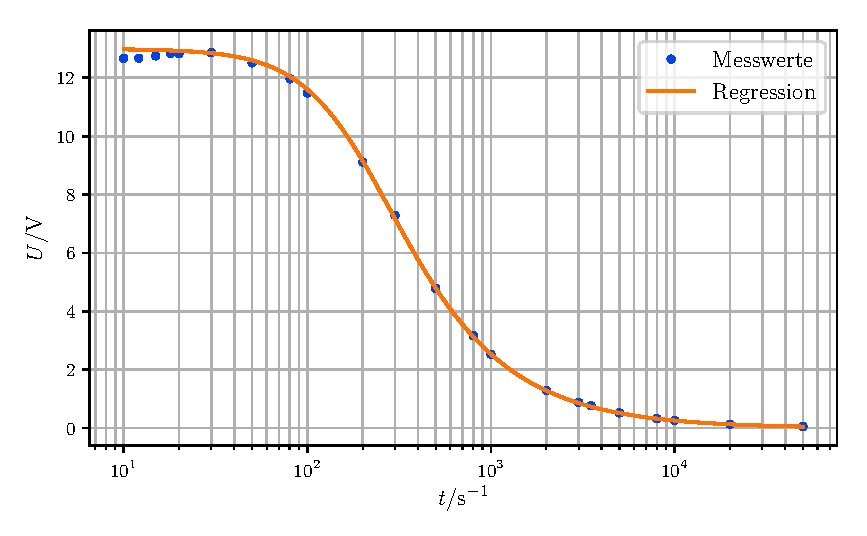
\includegraphics[width=\textwidth]{build/messung2.pdf}
    \caption{Messwerte.}
    \label{fig:plot2}
\end{figure}
%
\subsection{Frequenzabhängigkeit der Phasenverschiebung}
Aus der Messung zu Untersuchung der Frequanzabhängigkeit der Phasenverschiebung zwischen dem Generator und der Kondensatorspannung ergeben sich die in Tabelle \ref{tab:phase} aufgetragenen Werte. Aus den Messgrößen $a$ und $b$ wird nach Gleichung \eqref{eqn:abphase} der Phasenwinkel $\phi$ berechnen und ist ebenfalls angeführt.
%
\begin{table}[H]
    \caption{Messwerte der Phasenverschiebung.}
    \label{tab:phase}
    \centering
    \begin{tabular}{S[table-format=3.2(0)e0] S[table-format=5.2(0)e0] S[table-format=5.2(0)e0] S[table-format=1.3]}
        \toprule
            {$a/\si{\micro\second}$} & {$b/\si{\micro\second}$} & {$f/\si{\hertz}$} & {$\phi$} \\
        \midrule
        800.00  & 47400.00  & 21.09     & 0.106\\
        800.00  & 19980.00  & 50.08     & 0.252\\
        760.00  & 10000.00  & 100.00    & 0.478\\
        620.00  & 5000.00   & 200.00    & 0.779\\
        520.00  & 3330.00   & 300.00    & 0.981\\
        376.00  & 2000.00   & 500.00    & 1.181\\
        216.00  & 1000.00   & 1000.00   & 1.357\\
        116.00  & 499.84    & 2000.00   & 1.458\\
        68.00   & 285.60    & 3500.00   & 1.496\\
        48.00   & 200.88    & 5000.00   & 1.501\\
        24.00   & 99.84     & 10000.00  & 1.510\\
        12.20   & 50.00     & 20000.00  & 1.533\\
        4.88    & 20.01     & 50000.00  & 1.532\\
        \bottomrule
    \end{tabular}
\end{table}
\noindent
In Abbildung \ref{fig:plot3} sind die Messwerte und eine Theoriekurve nach Gleichung \eqref{eqn:phasetheorie} aufgetragen.
\begin{equation}
    \phi (\omega ) = \arctan (-\omega \, RC)
\end{equation}
Es wird mit Python/SciPy ein Curve-Fit erstellt, der Fit-Parameter ist hierbei $RC$.
\begin{figure}[H]
    \centering
    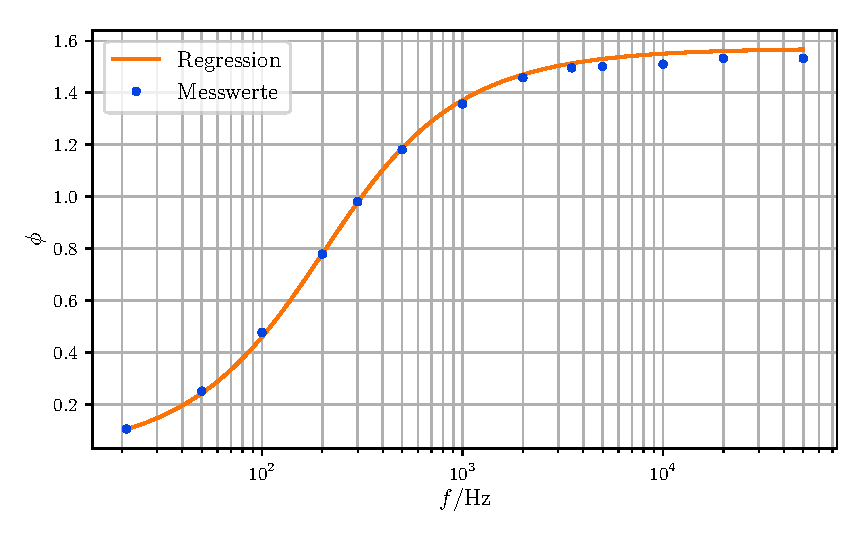
\includegraphics[width=\textwidth]{build/messung3.pdf}
    \caption{Messwerte und Curve-Fit der Phasenverschiebung.}
    \label{fig:plot3}
\end{figure}
\noindent
Es ergibt sich
\begin{equation}
    RC = \SI{-0.801\pm0.010e-3}{\second}.
\end{equation}
\noindent
\begin{figure}[H]
    \centering
    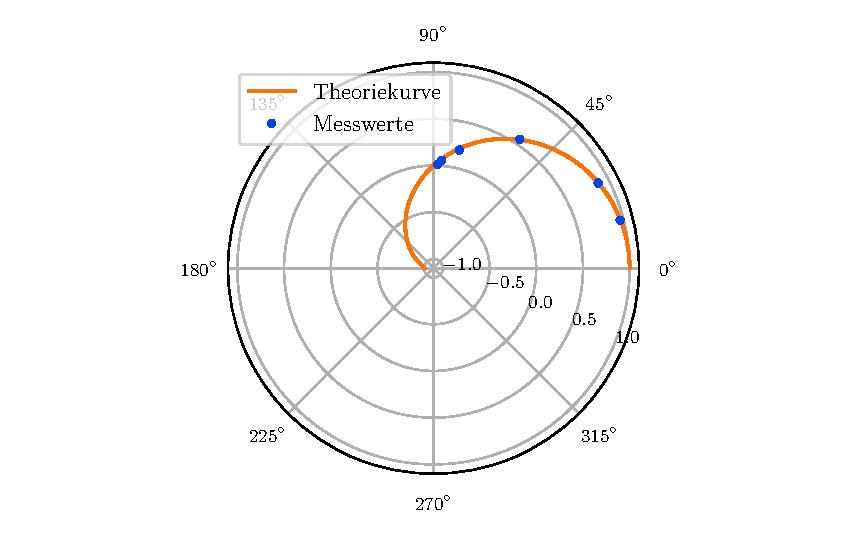
\includegraphics[width=\textwidth]{build/polar.pdf}
    \caption{Relative Amplitude gegen Phasenverschiebung.}
    \label{fig:polar}
\end{figure}
%
\subsection{RC-Glied als Integrator}
\begin{figure}[H]
    \centering
    \begin{minipage}{0.48\textwidth}
        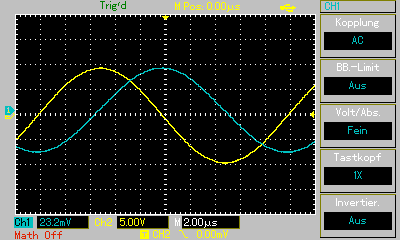
\includegraphics[width=\textwidth]{content/Grafiken/MAP001.png}
        \subcaption{.}
        \vspace{1em}
        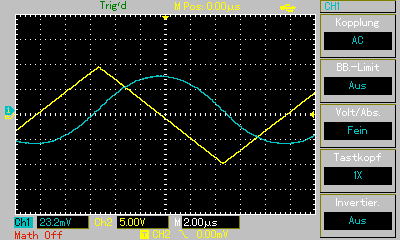
\includegraphics[width=\textwidth]{content/Grafiken/MAP002.png}
        \subcaption{.}
    \end{minipage}
    \hspace*{\fill}
    \begin{minipage}{0.48\textwidth}
        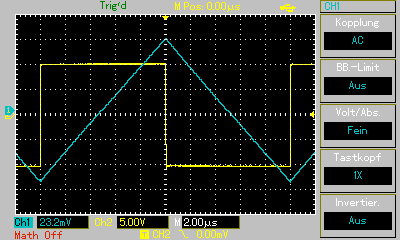
\includegraphics[width=\textwidth]{content/Grafiken/MAP003.png}
        \subcaption{.}
        \vspace{1em}
        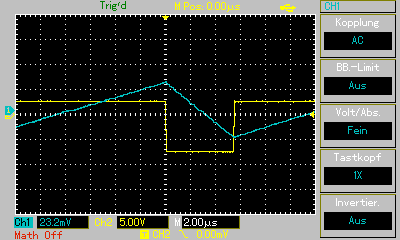
\includegraphics[width=\textwidth]{content/Grafiken/MAP004.png}
        \subcaption{.}
    \end{minipage}
    \caption{.}
\end{figure}
\noindent

\section{Diskussion}
\label{sec:Diskussion}
\begin{table}[H]
  \centering
  \begin{tabular}{S[table-format =1.3(4)]}
    \toprule
    {Relaxationszeit/\si{\milli\second}}\\
    \midrule
    0.813\pm0.009 \\
    0.801\pm0.010 \\
    0.789\pm0.018\\
    \bottomrule
  \end{tabular}
\end{table}
\noindent
Die Messergebnisse liegen innerhalb ihrer Toleranzen beieinander. Die Unsicherheiten selbst liegen im Bereich $<\SI{3}{\percent}$.
Als Fehlerquelle ist der Innenwiderstand des Generators zu beachten. Dieser hat einen Wert von $R_\text{i} = \SI{600}{\ohm}$. Verglichen mit dem gemessen Widerstand des RC-Glieds $R=\SI{8169}{\ohm}$ liegt dieser bei nur etwa $\SI{7}{\percent}$ und ist somit vernachlässigbar.


\printbibliography{}

\end{document}
